\documentclass[a4paper]{article}

\usepackage[portuguese]{babel}
\usepackage[utf8]{inputenc}
\usepackage{indentfirst}
\usepackage{graphicx}
\usepackage{verbatim}

\begin{document}

\setlength{\textwidth}{16cm}
\setlength{\textheight}{22cm}

\title{\Huge\textbf{Jogos de tabuleiro}\linebreak\linebreak\linebreak
\Large\textbf{Relatório 1ª Fase}\linebreak\linebreak

\includegraphics[height=6cm, width=7cm]{feup.pdf}\linebreak \linebreak
\Large{Mestrado Integrado em Engenharia Informática e Computação} \linebreak \linebreak
\Large{Base de dados}\linebreak
}

\author{\textbf{Grupo 601:}\\ Hugo Ari Rodrigues Drumond --- 201102900 \\  Ricardo Jorge Matos Figueiredo --- 201100687 \\ Gustavo Assis Freitas --- 200602187\\\linebreak\linebreak \\
 \\ Faculdade de Engenharia da Universidade do Porto \\ Rua Roberto Frias, 4200--65 Porto, Portugal \linebreak\linebreak\linebreak
\linebreak\linebreak\vspace{1cm}}
\maketitle
\thispagestyle{empty}

\newpage

%Decidimos elaborar uma base de dados para uma Empresa organizadora de \textit{Jogos de tabuleiro}.    \cite{creator}


%Descrever muito sumariamente (1-2 parágrafos) o trabalho que está a ser reportado

%\section{Introdução}

%Descrever os objectivos e motivação do trabalho.
%Todas as figuras devem ser referidas no texto. %\ref{fig:codigoFigura}

\section{Contexto}
Esta base de dados destina-se a um Salão de jogos que organiza jogos de Tabuleiro e foi desenvolvida, inicialmente, pensando num só jogo, o xadrez. Posteriormente, então, foi feita uma generalização. Em suma, são guardados os dados dos jogadores e dos torneios de uma dada temporada. Isto, possibilitará aos utilizadores da base de dados: rigor ao planear eventos, versatilidade, facilidade de registo, entre outros. Por exemplo, se eu quisesse organizar um torneio, em condições, iria ter saber à priori: os escalões, o jogo a que diz respeito, a temporada, as equipas inscritas e os patrocinadores. E registá-los em algum sítio para que depois possa associá-los, direta ou indiretamente, a uma partida e uma partida a equipas. A nossa base de dados tem como único propósito tornar esse \{pré,pós\}registo trivial.
%Para quem se destina, quem e que vai usar, 

\section{Conceitos Principais}
%Identificar as classes e falar um pouco sobre elas. As óbvias não é necessário.


%Identificar as classes e falar um pouco sobre elas. As óbvias não é necessário.
%jogador, país,equipa,formato,localpartida,escalão,jogo,temporada,torneio,patrocinador,partida e arbitro
%jogador:nome,email,dataNascimento,morada,telefone,pontos
%país: nome,extensão
%equipa: nome,
%Formato:
%Jogo: nome
%localPartida: morada,andar,sala,telefone
%escalão:nome
%temporada: ano,nome
%torneio: nome
%patrocinador: nome
%media: nome
As classes constituintes desta base de dados são:

\begin{itemize}

\item A classe "\textbf{Jogador}" é referente a cada jogador que participa no jogo e têm como atributos um nome(string), um email(string), uma data de nascimento(string), uma morada(string), um número de telefone(string) e os respectivos pontos(int). Um jogador pode fazer parte de várias equipas.

\item A classe "\textbf{País}", é referente a todos os países e está associado à nacionalidade quer do jogador quer do árbitro e ao local da partida. Tem como atributos um nome(string) e uma extensão(string). Um desses objetos estará associado a um só país.

\item A classe "\textbf{Equipa}", é referente a todas as equipas existentes no jogo e tem como atributo um nome(string). Uma equipa pode ser constituída por um só elemento, talvez um nome mais apropriado seria grupo.

\item A classe "\textbf{Formato}" refere-se ao tipo de torneio, por exemplo: todos contra todos, um contra todos, por equipas, etc. Guardando-se essa informação numa string chamada tipo.

\item A classe "\textbf{Jogo}" é referente ao tipo de jogo e tem como único atributo um nome(string) que pode ser damas, xadrez, monopólio, etc.

\item A classe "\textbf{Partida}" é onde se guarda a informação relativa a um duelo, data(string) e duração(inteiro).

\item A classe "\textbf{LocalPartida}" é referente ao local onde são feitas as partidas de cada torneio, tem como atributos uma morada(string), uma sala(string), e um telefone(string).

\item A classe "\textbf{Escalão}", é referente ao escalão do torneio, e tem como atributo o nome(string) do respectivo escalão. Um torneio poderá ter vários escalões.

\item A classe "\textbf{Temporada}" é referente à temporada em que é efectuado o torneio, tem como atributos o ano(string) da temporada e o nome(string). Um dado torneio só pode estar associado a uma temporada.

\item A classe "\textbf{Torneio}" poderá conter diversos escalões, mas só para um jogo, e tem como atributos o nome(string).

\item A classe "\textbf{Patrocinador}" refere-se aos possíveis patrocinadores da liga e à relação torneio, equipa e patrocinador e tem como atributos o nome(string) da respetiva associação/empresa patrocinadora. Decidimos criar uma relação ternária entre torneio, equipa e patrocinador porque para uma equipa poderá ter patrocinadores diferentes consoante um dado torneio.

\item A classe "\textbf{Arbitro}" é referente ao arbitro, e possui os campos: nome e a data de nascimento.
\end{itemize}

Todos os atributos têm de ser preenchidos (not NULL), excluindo: Jogador::email e localPartida::\{andar,sala\}.

%Prof favor completem com um texto melhor que explique os relacionamentos das classes mais dificeis 

\section{Diagrama de classes UML}
%Incluir todas as restrições, digitalizar o diagrama ou fazer num programa qualquer. Incluir notas.

\begin{center}
  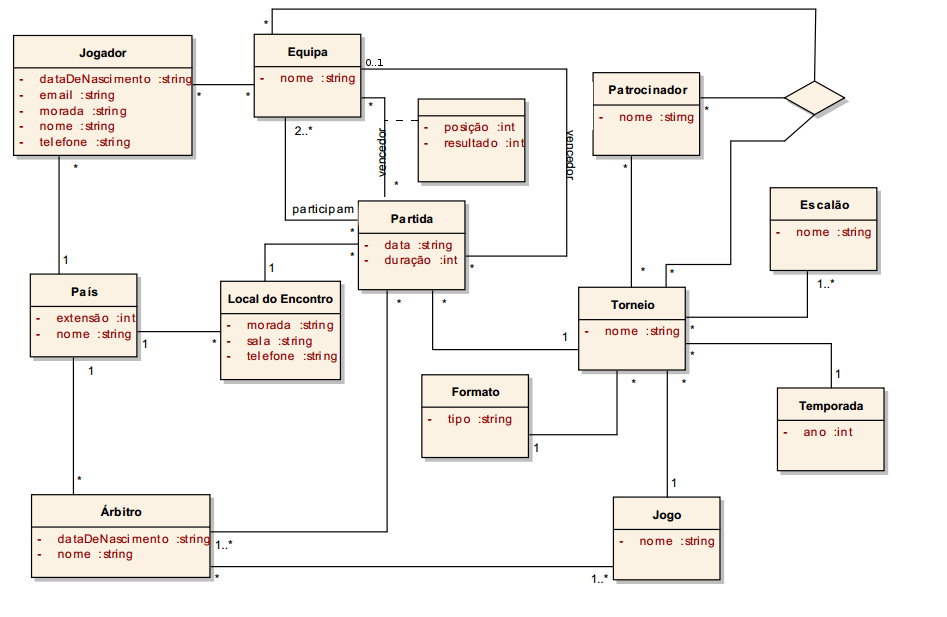
\includegraphics[scale=0.70]{UML.png}
  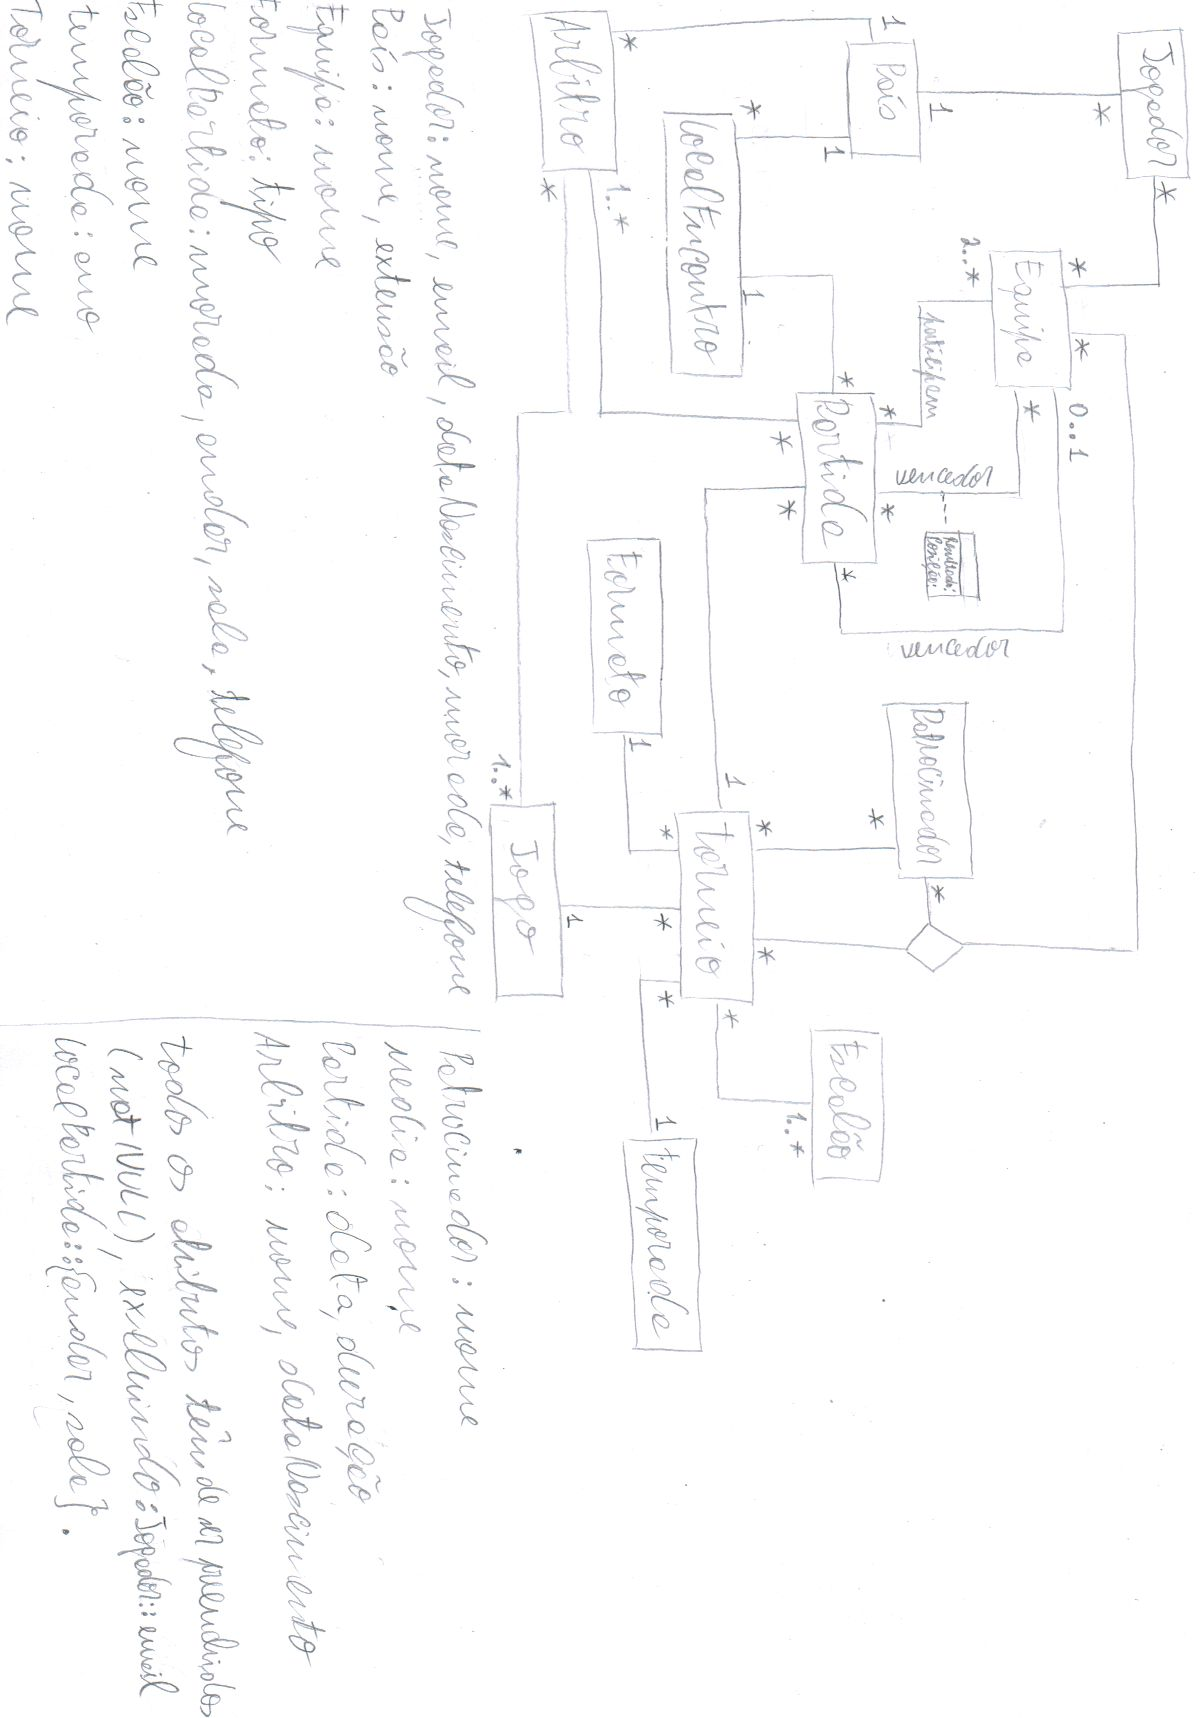
\includegraphics[scale=0.83]{BDAD_DIAGRAMA.jpeg}
\end{center}

\clearpage
\addcontentsline{toc}{section}{Bibliografia}
\renewcommand\refname{Bibliografia}
\bibliographystyle{plain}
\bibliography{myRefs}

\end{document}
